\documentclass[tikz,border=4pt]{standalone}
\usepackage{pgfplots}
\usepackage{times}
\pgfplotsset{compat=1.18}
\begin{document}
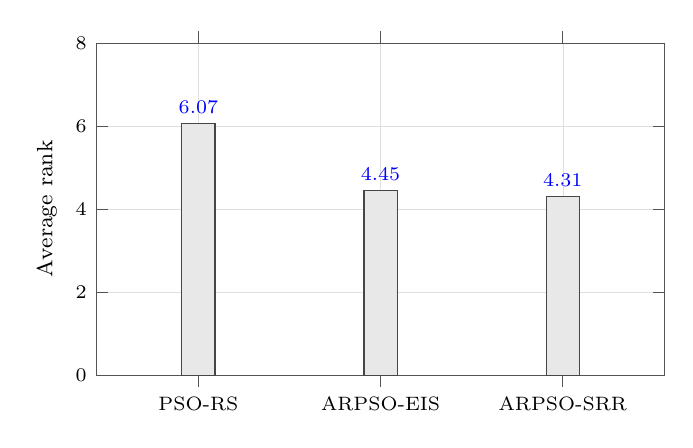
\begin{tikzpicture}
\begin{axis}[
    width=88mm,
    height=58mm,
    ybar,
    bar width=12pt,
    ymin=0,
    ymax=8,
    ylabel={Average rank},
    symbolic x coords={PSO-RS,ARPSO-EIS,ARPSO-SRR},
    xtick=data,
    xticklabel style={font=\scriptsize},
    tick label style={font=\scriptsize},
    label style={font=\footnotesize},
    nodes near coords,
    every node near coord/.append style={font=\scriptsize},
    grid=major,
    grid style={line width=.15pt, draw=gray!25},
    axis line style={gray!65!black},
    tick style={gray!65!black},
    enlarge x limits=0.28,
    point meta=explicit symbolic,
]
\addplot+[draw=gray!55!black, fill=gray!18] coordinates {
(PSO-RS,6.07) [6.07]
(ARPSO-EIS,4.45) [4.45]
(ARPSO-SRR,4.31) [4.31]
};
\end{axis}
\end{tikzpicture}
\end{document}
